Here, we evaluate our approach on  a numerical simulator by focusing on three questions: \textbf{(Q1)} Can our approach closely approximate Nash equilibrium and generate competitive behavior? \textbf{(Q2)} How do hyper-parameters like the discount factor $\gamma$ and the amount of data used to learn the \(\alpha\)-potential function affect the performance? \textbf{(Q3)} How does our approach compare against common baselines?

\vspace{1mm}
\noindent \textbf{Experimental Setup:} We generate a dataset of 4000 races, each lasting 50 seconds, conducted with randomly chosen policy parameters and involving 3 cars. This dataset is used to first train value function estimators $V^1$, $V^2$, and $V^3$ for each of the cars. These are then used to learn $\Phi$ using \eqref{eq: LinearSemiInfiniteFormulation}. To maximize the learned potential function, we use gradient ascent with a learning rate of $10^{-4}$ and warm-start by using the solution from the previous time step.


% FIGS HERE
\begin{figure}
    \centering
    \begin{subfigure}{} 
        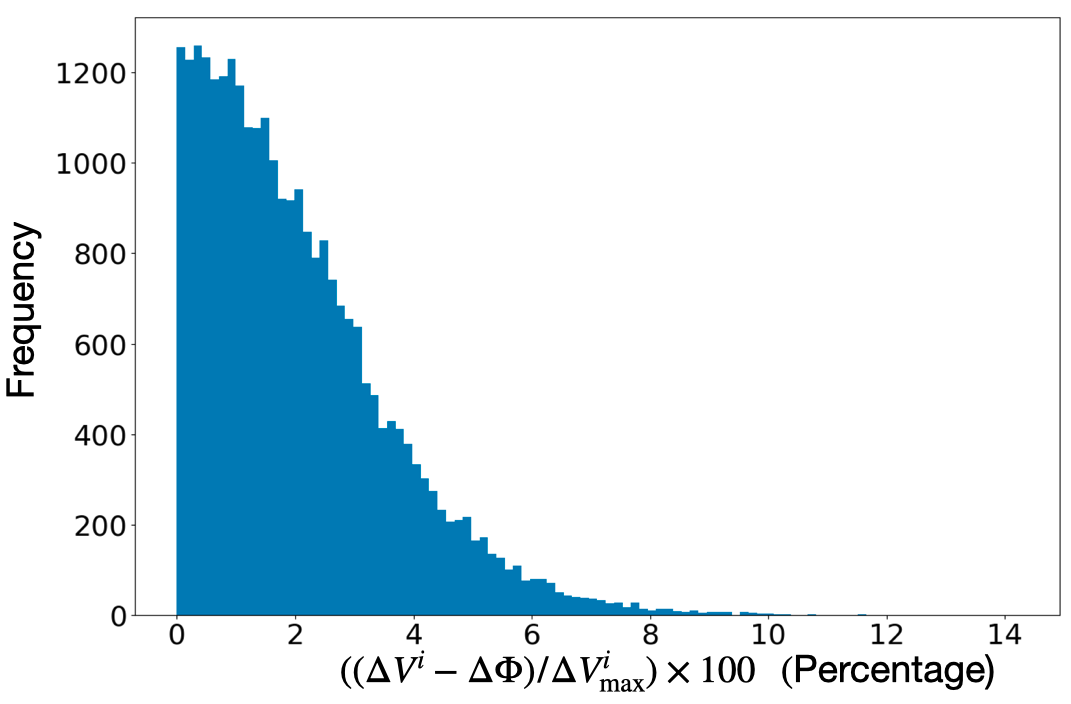
\includegraphics[width=5cm]{Figures/Fig_Keynote/ds_new_keynote.png}
        % {Figures/ds_new.png}
        \label{subfig:ds}
    \end{subfigure}
    \begin{subfigure}{} 
        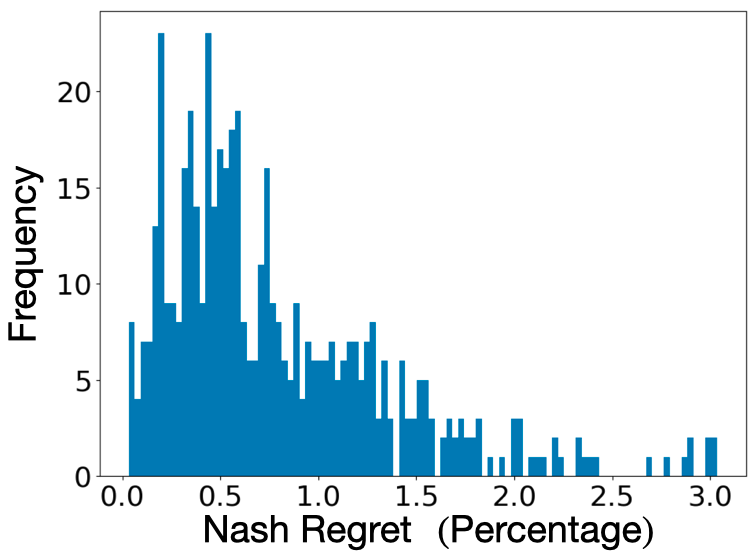
\includegraphics[width=4.3cm]{Figures/Fig_Keynote/regrets_new_keynote.png}
        % {Figures/regrets_new.png}  
        \label{subfig:regrets}
    \end{subfigure}
    \caption{Histogram of (a) Relative approximation gap of potential function (b) Nash regret}
    \label{fig:regrets}
\vspace{-7mm}  
\end{figure}

\vspace{-5mm}
\subsection{Competitive Behavior by Approximating Nash Equilibrium}
\vspace{-2mm}
We observe that the approximation gap of the learned potential function is small. As shown in Figure~\ref{fig:regrets}(a), the approximation gap across all states and policy parameters used in the training samples remains within 10\% of the value function's range, with a median gap of approximately 2\%.  
Next, we demonstrate that the optimization solver effectively computes the maximizer of the potential function, leading to a lower Nash approximation error. In particular, Figure~\ref{fig:regrets}(b) shows the \textit{Nash regret} for the ego agent, defined as  
\(
\max_{\theta^i} V^i(\mathbf{x}, \theta^i, \theta^{\ast,-i}) - V^i(\mathbf{x}, \theta^{\ast,i}, \theta^{\ast,-i}),
\)  
where \(\theta^\ast\) is the optimizer of the potential function with the starting state \(\mathbf{x}\). The regret is plotted for different game states during a race, and we observe that it remains within 3\% of the range of the value function.  
In summary, Figure~\ref{fig:regrets} highlights that the dynamic game admits an \(\alpha\)-potential function with small \(\alpha\), and that we accurately compute a near-optimal solution to the potential function.



Next, in Figure~\ref{fig:potential_values}, we show that, by fixing all policy parameters but one, the parameter that (approx.) maximizes potential function  
% potential function maximized over different parameters of the ego agent
generates a trajectory that maximizes progress along the track over the next 5 seconds. This is highlighted by yellow diamond in Figure \ref{fig:potential_values}.


\begin{figure}
    \centering
    \begin{subfigure}{} 
        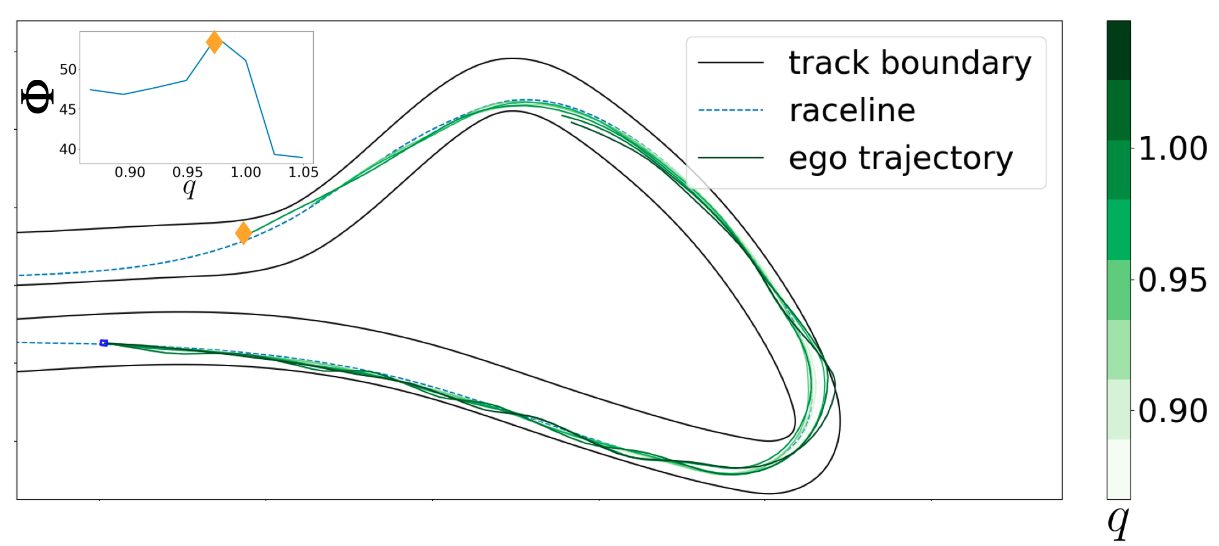
\includegraphics[width=5.5cm]{Figures/Fig_Keynote/p_q_new_keynote.png}
        % {Figures/p_q_new.png}    
        % \label{subfig:p_q}
    \end{subfigure}
    \begin{subfigure}{} 
        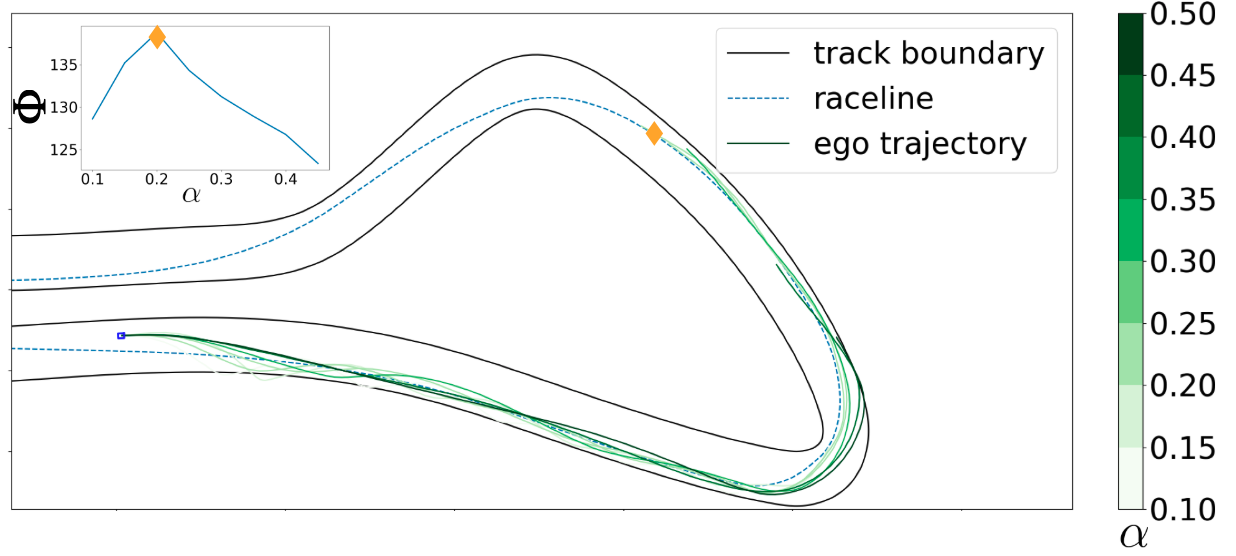
\includegraphics[width=5.5cm]{Figures/Fig_Keynote/p_alpha_new_keynote.png}
        % {Figures/p_alpha_new.png}
        % \label{subfig:p_alpha}
    \end{subfigure}\\
    \begin{subfigure}{} 
        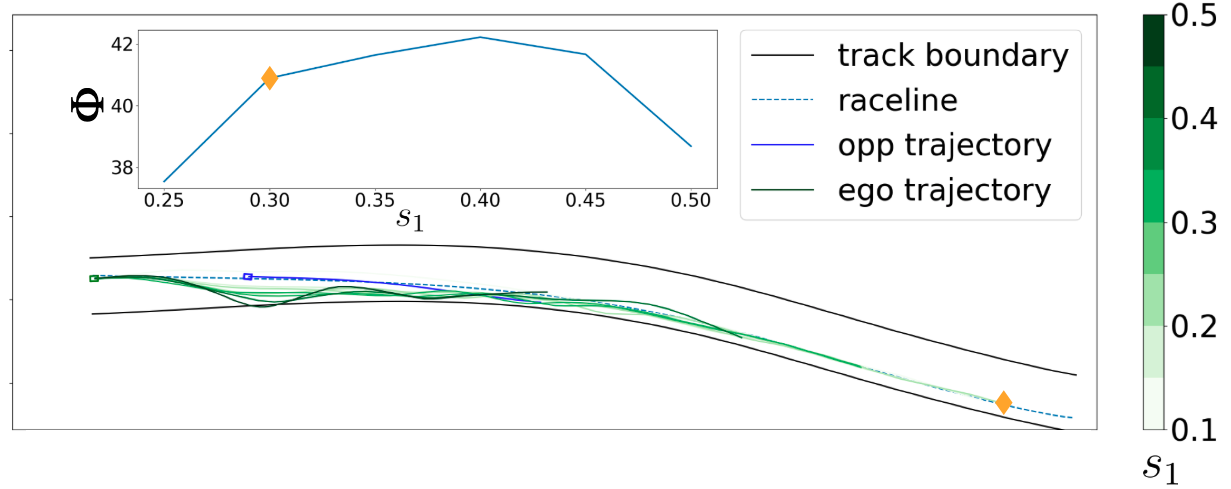
\includegraphics[width=5.5cm]{Figures/Fig_Keynote/p_s1_new_keynote.png}
        % {Figures/p_s1_new.png}
        % \label{subfig:p_s1}
    \end{subfigure}
    \begin{subfigure}{} 
        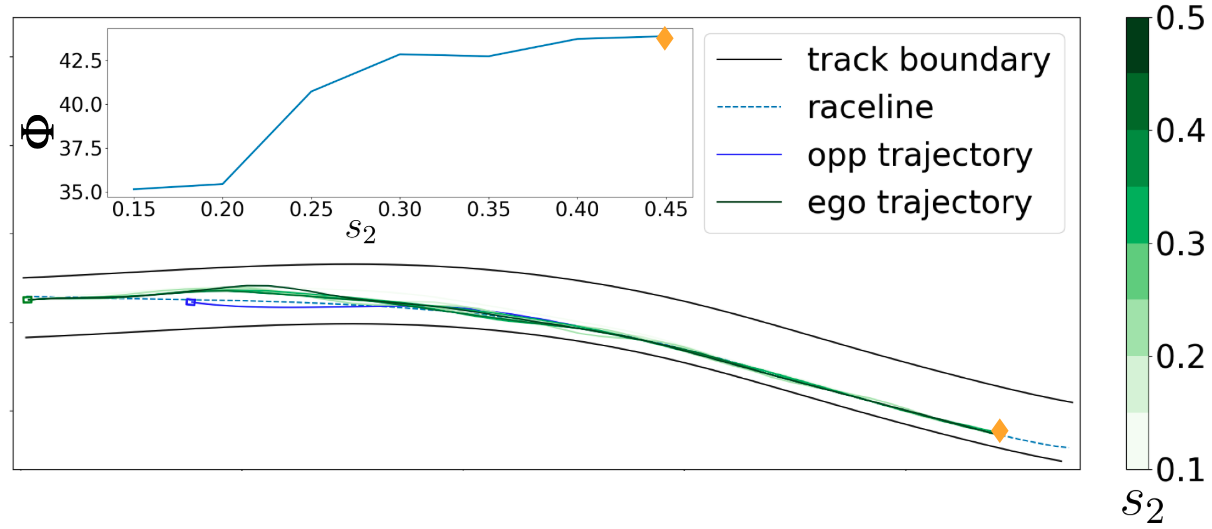
\includegraphics[width=5.5cm]{Figures/Fig_Keynote/p_s2_new_keynote.png}
        % {Figures/p_s2_new.png}
        % \label{subfig:p_s2}
    \end{subfigure}
    \begin{subfigure}{} 
        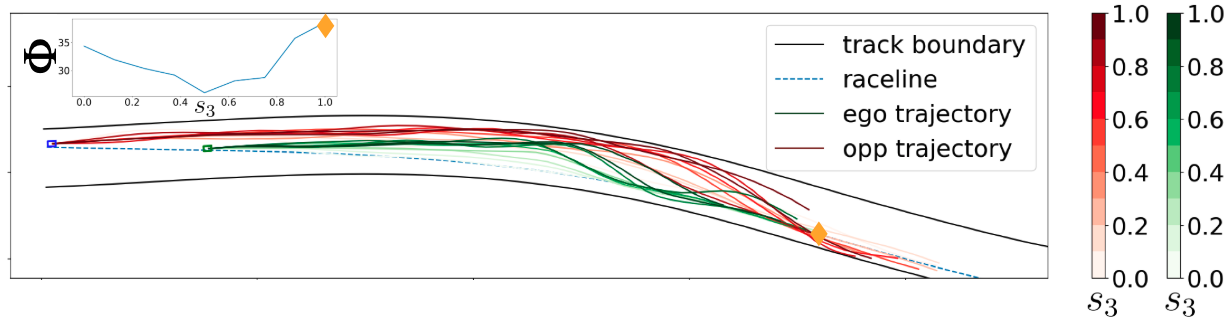
\includegraphics[width=8cm]{Figures/Fig_Keynote/p_s3_new_keynote.png}
        % \label{subfig:p_s3}
    \end{subfigure}
    \caption{Potential values and the trajectories at a given joint state for different (a) $q$ (b) $\zeta$ (c) $s_1$ (d) $s_2$ (e) $s_3$ of only the ego agent. We only denote 2 players here (only 1 player for (a) and (b)) and the 3rd player is far away from this position to not affect any players. Additionally, for ease of readability, we only show the impact of variation in trajectory of other player in response to \textsf{ego} in (e) as such deviations are not significant in (c) and (d).
    % We see that the trajectory that makes most progress correspond to approximate maximizing parameter for potential function (see yellow diamond).
    }
    \label{fig:potential_values}
    \vspace{-6mm}
\end{figure}

% \begin{figure}
%     \centering
%     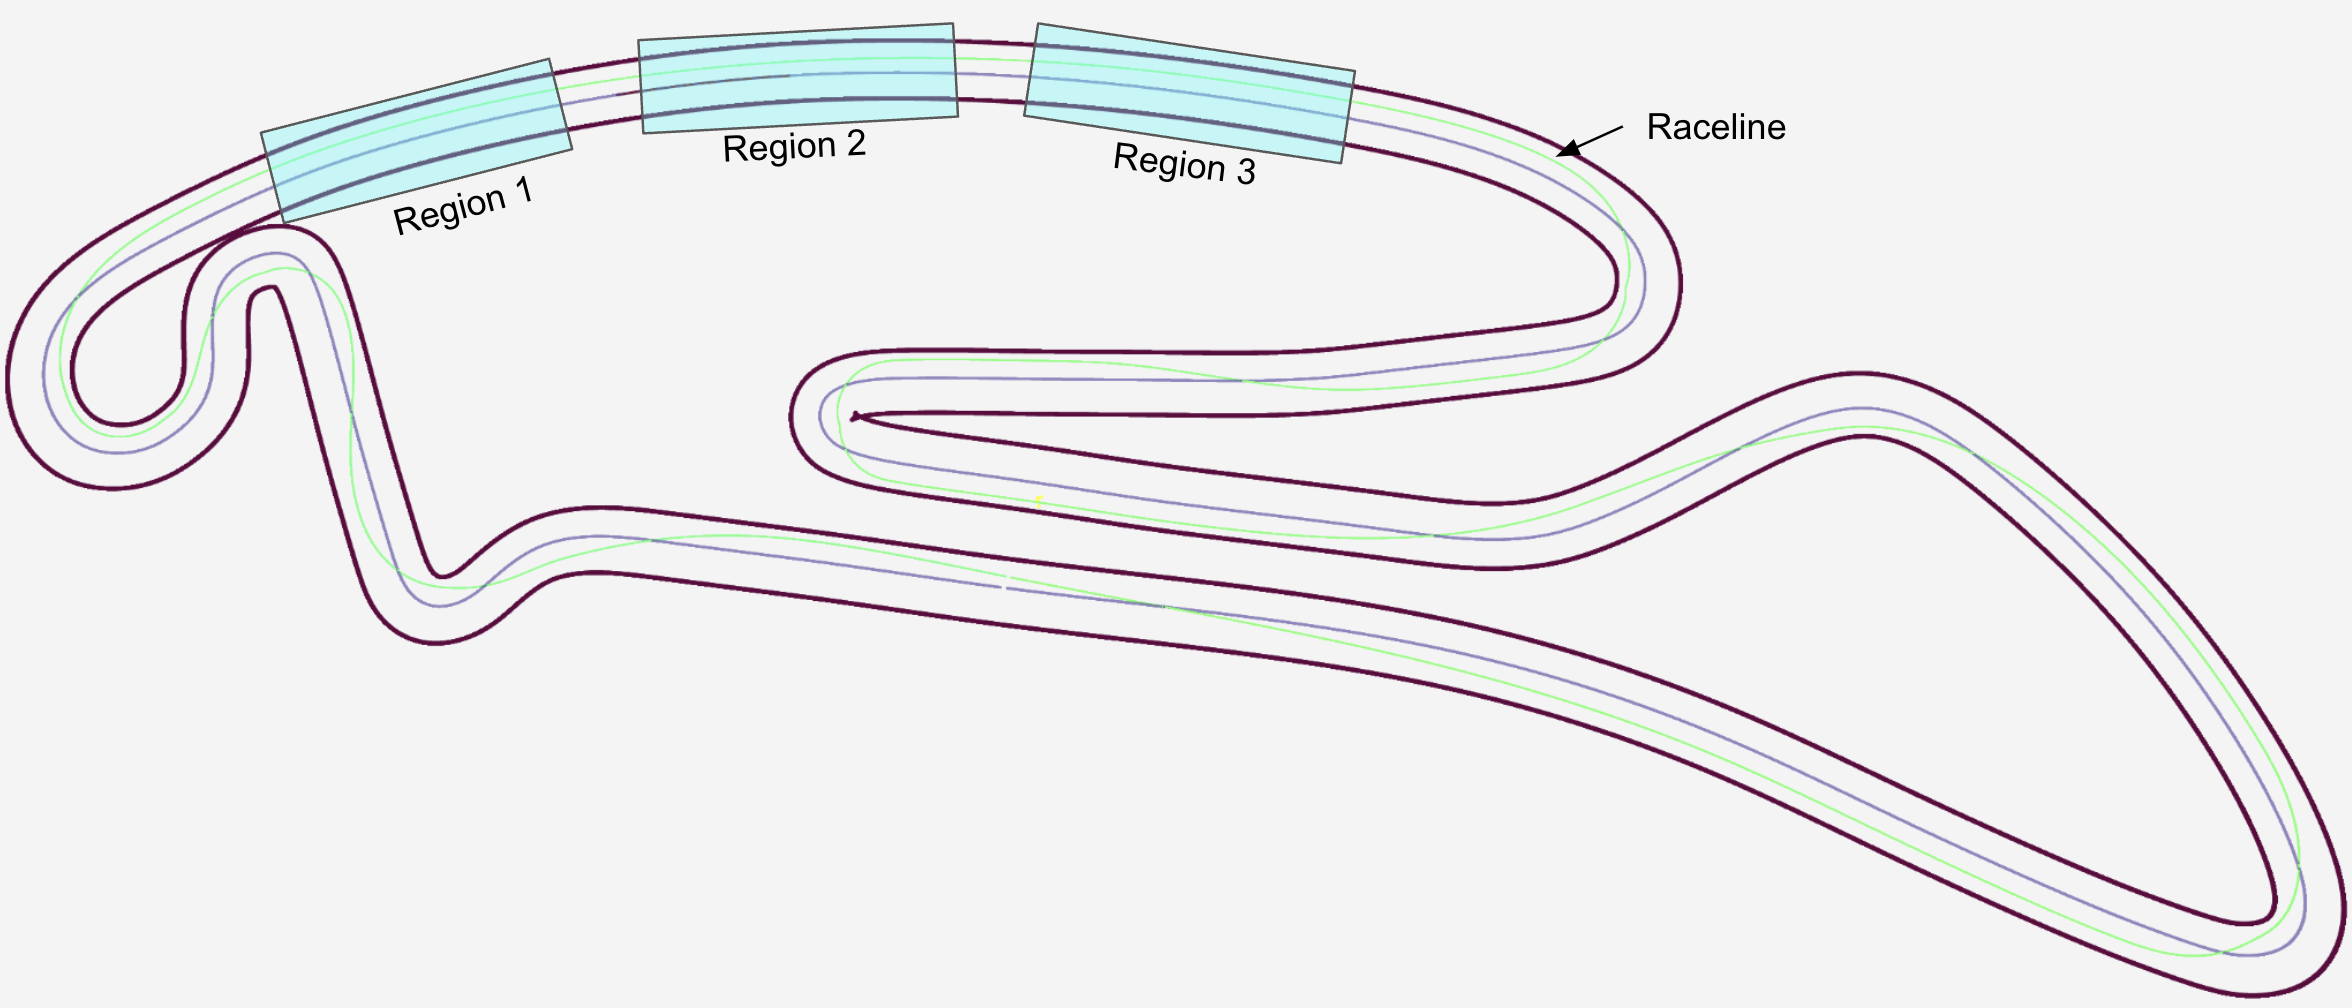
\includegraphics[width=0.5\linewidth]{Figures/track.png}
%     \caption{Regrets histogram for a race. Maximum value of}
%     \label{fig:regrets}
% \end{figure}



\vspace{-5mm}
\subsection{Performance Comparison}
\vspace{-2mm}
To address questions \textbf{Q2} and \textbf{Q3}, we conduct 99 races involving three agents: \textsf{ego}, \(\textsf{O}_1\), and \(\textsf{O}_2\). Here, \textsf{ego} represents the agent using our proposed algorithm, while \(\textsf{O}_1\) and \(\textsf{O}_2\) are opponents employing other algorithms. In this study, we vary the opponents' algorithms and compute the winning fraction for the \textsf{ego} car. A visualization of the track used in the study, along with the computed optimal race-line, is provided in the supplementary material (Figure~4).
The starting positions for the races are taken from three regions (denoted by \(\textsf{R}_1\), \(\textsf{R}_2\), and \(\textsf{R}_3\)), such that \(\textsf{R}_1\) is the furthest ahead on the track, followed by \(\textsf{R}_2\), and then \(\textsf{R}_3\), as shown in the supplementary material (Figure~4). We perform 33 races, each with the \textsf{ego} agent starting in \(\textsf{R}_1\), \(\textsf{R}_2\), or \(\textsf{R}_3\). Also, \(\textsf{O}_1\) is always placed ahead of \(\textsf{O}_2\).

For the \textsf{ego}, we use a discount factor \(\gamma = 0.99\) and a training dataset comprising \(4000\) races. Below, we summarize five different opponent strategies for \(\textsf{O}_1\) and \(\textsf{O}_2\):

\noindent \((i)\) \textbf{Case I:} Opponents trained with a lower discount factor than \textsf{ego} (i.e., \(\gamma = 0.98\)); 

\noindent \((ii)\) \textbf{Case II:} Opponents trained with a higher discount factor than \textsf{ego} (i.e., \(\gamma = 0.995\));

\noindent \((iii)\) \textbf{Case III:} Opponents trained using fewer simulated races than \textsf{ego} (i.e., \(400\) races);

\noindent \((iv)\) \textbf{Case IV:} Opponents use the \textit{Iterated Best Response} (IBR) algorithm \footnote{The IBR algorithm used here is representative of the methods developed in \cite{spica2020real, Wang2020MultiagentSE}, though it may not be an exact implementation, as the original code is not publicly available.}, which computes the best response of opponents in round-robin for a fixed number of rounds (i.e., 6), with a planning horizon\footnote{Choice of hyperparameters is such that it roughly takes the same compute time as our approach.} of length \(2s\);

\noindent \((v)\) \textbf{Case V:} Opponents trained using self-play RL\footnote{Here, self-play RL represents the approach in \cite{thakkar2022hierarchical}, excluding the high-level tactical planner.}. We use a similar observation and reward as used in \cite{thakkar2022hierarchical} and train with \(2M\) steps.


% For the \textsf{ego}, we use a discount factor \(\gamma = 0.99\) and a training dataset comprising \(4000\) races. Below, we summarize five different opponent strategies for \(\textsf{O}_1\) and \(\textsf{O}_2\): \((i)\) \textbf{Case I:} Opponents trained with lower discount factor than \textsf{ego} (i.e., $\gamma=0.98$); \((ii)\) \textbf{Case II:} Opponents trained with higher discount factor than \textsf{ego} (i.e., $\gamma=0.995$); \((iii)\) \textbf{Case III:}  Opponent trained using less simulated race data than \textsf{ego} (i.e., $400$ races); \((iv)\) \textbf{Case IV:} Opponent using \textit{Iterated Best Response} (IBR) algorithm (representative of the algorithms discussed\footnote{Note that this may not be the exact implementation of \cite{spica2020real} as the code is not open-sourced}  in \cite{spica2020real, Wang2020MultiagentSE}), that computes best response of opponents in round-robin for a fixed number of rounds ($6$), with planning horizon\footnote{We select horizon length as $2s$ and no of rounds as $6$ such that it roughly takes similar compute time to our approach.} of length \(2s\). \((v)\) \textbf{Case V:} Opponent trained using self-play RL (representative of \cite{thakkar2022hierarchical} sans the high-level tactical planner proposed in their work). We use a similar observation and reward as used in \cite{thakkar2022hierarchical} and train with $2M$ steps. 

% [{\color{magenta} Number of IBR Updates?}]
% \begin{enumerate} 
    % \item 
    % This is to prove a point that lower discount factor will enable learning potential function for short horizon which would lead to a myopic agent looking to optimize for short-term gains
    % {\color{red}\item \textbf{Opponent with high $\gamma$}: We also race against our approach with high discount factor $\gamma=0.995$. }
    % The potential function optimization will thus lead to a farsighted agent but at the cost of more restricted policy space}
    % \item \textbf{Opponent trained using less data}: For this setting, we only train potential function $\Phi$ estimator on $400$ races. 
    % This is to show that more training data helps in learning a more accurate potential function
    % \item \textbf{Opponent using Iterated Best Response (IBR)}: This is representative approach to \cite{spica2020real} \cite{Wang2020MultiagentSE} that directly aims at solving nash equilibrium for a finite horizon with the same one-step utility as here. We use horizon length as $2s$ such that it roughly takes similar compute time to our approach. It is important to note here that this may not be the exact and best implementation of \cite{spica2020real} as the code is not open-sourced 
    % \item \textbf{Opponent trained using self-play RL}: This is representative approach to \cite{wurman2022outracing} and \cite{thakkar2022hierarchical} sans the high-level tactical planner as proposed in the work. We use a similar observation and reward as used in \cite{thakkar2022hierarchical} and train the approach with $2M$ steps. 
% \end{enumerate}



\noindent The number of races won for all cases are provided in Table \ref{tab:3_agents}, where we see that \textsf{ego} agent trained using our approach has superior performance in comparison to all other opponent strategies.  

\vspace{1mm}
\noindent \textbf{Performance Variation with Hyperparameters (\textbf{Cases I–III}).}
The \textsf{ego} car outperforms opponents with lower discount factors (\textbf{Case I}) because lower discount factors lead to more myopic behavior, causing opponents to prioritize short-term progress over long-term track performance. Similarly, the \textsf{ego} car also outperforms opponents with higher discount factors (\textbf{Case II}) as higher discount factors increase the "effective horizon" of the game, which requires significantly more data to accurately approximate the value and potential functions.
Furthermore, the \textsf{ego} car has superior performance against opponents trained with less data of only $400$ races (\textbf{Case III}), as more data enables the learning of a more accurate \(\alpha\)-potential function.



\begin{table}[htbp] 
\centering
\begin{tabular}{|l|c|c|c|}
\hline
\textbf{Racing Scenario}              & \textbf{\# wins (ours)} & \textbf{\# wins ($\textsf{O}_1$)} & \textbf{\# wins ($\textsf{O}_2$)} \\ \hline
% {\color{red}MPC with random params}          & 78    & 12 &  9                   \\ \hline
% Opponents with low $\gamma$    
% \textbf{Case I} (Opponents with random policy parameters) & 84    & 9 & 6                   \\ \hline
\textbf{Case I} (Opponents with low $\gamma$) & 61    & 28 & 10                   \\ \hline
% Opponents with high $\gamma$  
\textbf{Case II} (Opponents with high $\gamma$)
& 52    & 40 & 7                   \\ \hline
% Opponents trained with less data    
\textbf{Case III} (Opponents trained with less data)
& 76    & 16 & 7  \\ 
\hline
% Opponent trained using IBR   
\textbf{Case IV} (Opponents using IBR)
& 73    & 22 & 4                   \\ \hline
% Opponent trained using self-play RL          
\textbf{Case V} (Opponents trained using self-play RL)
& 91    & 7 & 1                    \\ \hline
\end{tabular}
\caption{Outcomes of 99 races conducted between 3 cars under three different initial positions}
% :- a) ours $>$ $\textsf{O}_1$ $>$ $\textsf{O}_2$ b) $\textsf{O}_1$ $>$ ours $>$ $\textsf{O}_2$ c) $\textsf{O}_1$ $>$ $\textsf{O}_2$ $>$ ours, 33 races each. $\textsf{O}_1$ and $\textsf{O}_2$ are just 2 instances of the same opponent. 
% Videos of representative races in each scenario is at \href{https://sastry-group.github.io/alpha-RACE/}{\small https://sastry-group.github.io/alpha-RACE/}.}
\label{tab:3_agents}
\vspace{-3mm}
\end{table}


% \begin{table}[htbp] 
% \centering
% \begin{tabular}{|l|c|c|}
% \hline
% \textbf{Racing Scenario}              & \textbf{\# wins (ours)} & \textbf{\# wins (Opp)} \\ \hline
% % {\color{red}MPC with random params}          & 78    & 12 &  9                   \\ \hline
% % Opponents with low $\gamma$    
% \textbf{Case I} (Opponent with random policy parameters) & 92    & 8                   \\ \hline
% \textbf{Case II} (Opponent with low $\gamma$) & 69    & 31                   \\ \hline
% % Opponents with high $\gamma$  
% \textbf{Case III} (Opponent with high $\gamma$)
% & 72    & 28                   \\ \hline
% % Opponents trained with less data    
% \textbf{Case IV} (Opponent trained with less data)
% & 84    & 16   \\ 
% \hline
% % Opponent trained using IBR   
% \textbf{Case V} (Opponent using IBR)
% & 86    & 14                   \\ \hline
% % Opponent trained using self-play RL          
% \textbf{Case VI} (Opponent trained using self-play RL)
% & 97    & 3                    \\ \hline
% \end{tabular}
% \caption{Outcomes of 99 races conducted between 3 cars under three different initial positions
% % :- a) ours $>$ $\textsf{O}_1$ $>$ $\textsf{O}_2$ b) $\textsf{O}_1$ $>$ ours $>$ $\textsf{O}_2$ c) $\textsf{O}_1$ $>$ $\textsf{O}_2$ $>$ ours, 33 races each. $\textsf{O}_1$ and $\textsf{O}_2$ are just 2 instances of the same opponent. 
% Videos of representative races in each scenario is at \href{https://sites.google.com/view/game-theoretic-racing}{\small https://sites.google.com/view/game-theoretic-racing}.}
% \label{tab:2_agents}
% % \vspace{-2mm}
% \end{table}

% We also win more number of races with more myopic opponent (i.e., with low \(\gamma\)). This is because with low $\gamma$, the agent tends to look for more short term gains but suffers in long term. Finally with higher $\gamma$, the trained potential function is far-sighted but the policy space is more restricted and reliant on the policy parametrization for longer horizon. Hence, a balance of far-sightedness and more expressive policy space is necessary in choosing $\gamma$. With more expressive policy parametrization, higher $\gamma$ could do better. 

\begin{figure}
    \centering
    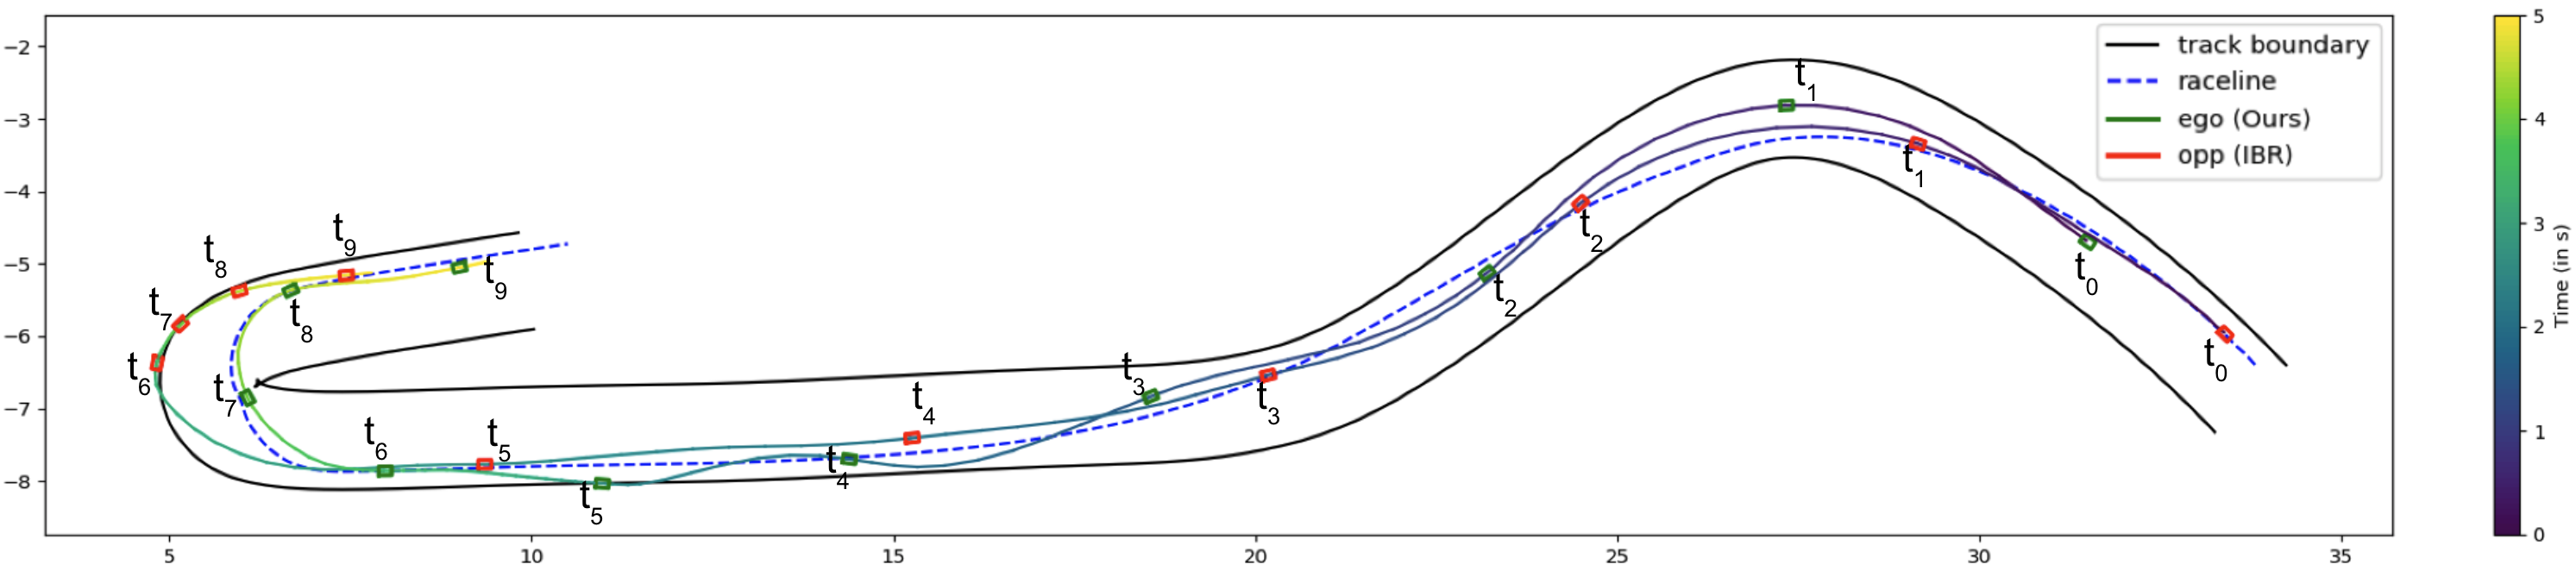
\includegraphics[width=.9\linewidth]{Figures/race_eg2_timestamps.png}
    \caption{Example overtake in a race MPC vs IBR. Opponent (IBR) overtakes from $t_4$ to $t_5$ but later suffers at the turn from $t_5$ to $t_9$ when the Ego agent (Ours) overtakes back to re-claim it's position}
    \label{fig:race_eg}
    \vspace{-6mm}
\end{figure}

% \vspace{1mm}
\noindent \textbf{Comparison with opponents using IBR (Case IV).} Our approach surpasses IBR for two key reasons. First, IBR may not always converge to a Nash equilibrium. Second, IBR's real-time computation is often restricted to local planning with a short \(2s\) horizon, as noted in \cite{spica2020real, wang2019bgame}. In contrast, competitive racing demands prioritizing a global racing line to optimize long-term performance, with strategic deviations for overtaking or blocking rather than short-term gains. This distinction is highlighted in Figure~\ref{fig:race_eg}, where the IBR player achieves higher straight-line speeds to overtake but struggles in turns due to aggressive braking. While our implementation is not a direct comparison with \cite{spica2020real}, our approach supports longer-horizon planning for real-time control by leveraging offline potential function learning. This is achieved by constraining the policy space to primitive behaviors, closely aligning with practical racing strategies.

\noindent \textbf{Comparison with opponents using self-play RL (Case V).}
Our approach also outperforms opponents trained via self-play RL. While we do not claim an optimized implementation of self-play RL—acknowledging potential improvements through further training, hyperparameter tuning, or tactical enhancements as in \cite{thakkar2022hierarchical}—our method offers clear advantages. It delivers interpretable solutions grounded in realistic racing strategies and approximation guarantees to a Nash equilibrium in races with more than 2 cars. In contrast, self-play RL often requires additional insights to develop effective policies. For example, \cite{thakkar2022hierarchical} showed that augmenting self-play RL with high-level tactical plans significantly enhances policy learning.

